\chapter{Prueba de concepto}

En este capítulo se va a hablar de una pequeña prueba de concepto para ver el funcionamiento de todas las APIs y herramientas conjuntamente.

Inicialmente, se establece una arquitectura de desarrollo, en la que se define el papel de cada API y herramienta.

Por último, se realiza una explicación del funcionamiento de la prueba de concepto, así como una vista de los resultados finales.


\section{Arquitectura}
\label{sec:arquitectura}

La arquitectura de la demostración muestra los diferentes elementos que la componen, así como las interacciones entre ellos para el intercambio de datos.

A continuación vemos una explicación de cada elemento perteneciente a la demo y que componente lleva a cabo esa acción:

\begin{itemize}
	\item \textbf{Operation Support System (OSS):} representa el papel de un operador que despliega un servicio gracias a una aplicación. El operador es emulado mediante Net2Plan, más concretamente por su plugin de \textit{NFV Management} (ver sección \ref{sec:nfvplugin}).
	
	\item \textbf{NFV Orchestrator (NFV-O):} representa el papel de una aplicación que se encarga de gestionar la infraestructura de virtualización necesaria para instanciar diferentes máquinas virtuales. ETSI-OSM (ver \ref{sec:osm}) es el encargado de dicha función.
	
	\item \textbf{Virtual Infrastructure Managers (VIMs):} son los encargados de instanciar y alojar las diferentes máquinas virtuales pertenecientes a los VNF. OpenStack (ver \ref{sec:openstack}) es quien realiza este papel.
	
	\item \textbf{Red de Transporte:} la red de transporte es emulada mediante Mininet (ver \ref{sec:mininet}) para establecer flujos de paquetes entre las diferentes VNFs de una Service Chain.
	
	\item \textbf{Controlador SDN:} la red de transporte es controlada por una instancia de ONOS (ver \ref{sec:onos}) mediante el envio de paquetes Openflow (ver \ref{subsec:openflow}) a los diferentes switches de la red.
	
	\item \textbf{Latency-Aware Service Chain Computation Element (LA-SCCE):} Se encarga de decidir el camino a seguir para atravesar una secuencia de VNFs que cumpla con los requisitos de latencia máxima. Este papel lo representa la extensión de Net2Plan mediante la ejecución de un algoritmo de \textit{NFV Placement}. 
\end{itemize}

En la figura \ref{fig:esquemademo} se puede observar un esquema de la arquitectura, en el que se incluyen todos los elementos explicados anteriormente, y hace más fácil de entender como interactúan entre sí los componentes:

\begin{figure}[!ht]
	\centering
	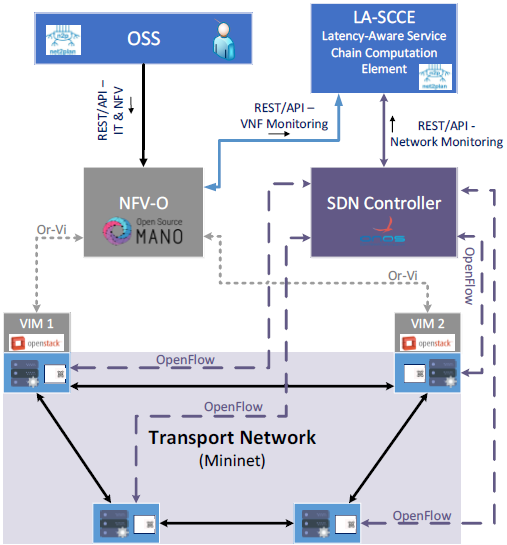
\includegraphics[width=0.7\linewidth]{imagenes/esquema_demo}
	\caption{Arquitectura de la Prueba de Concepto}
	\label{fig:esquemademo}
\end{figure}

\clearpage

\section{Funcionamiento}

A continuación se explican los diferentes pasos que se realizan para llevar a cabo la prueba de concepto y que APIs intervienen en cada uno de ellos:

\begin{figure}[!ht]
	\centering
	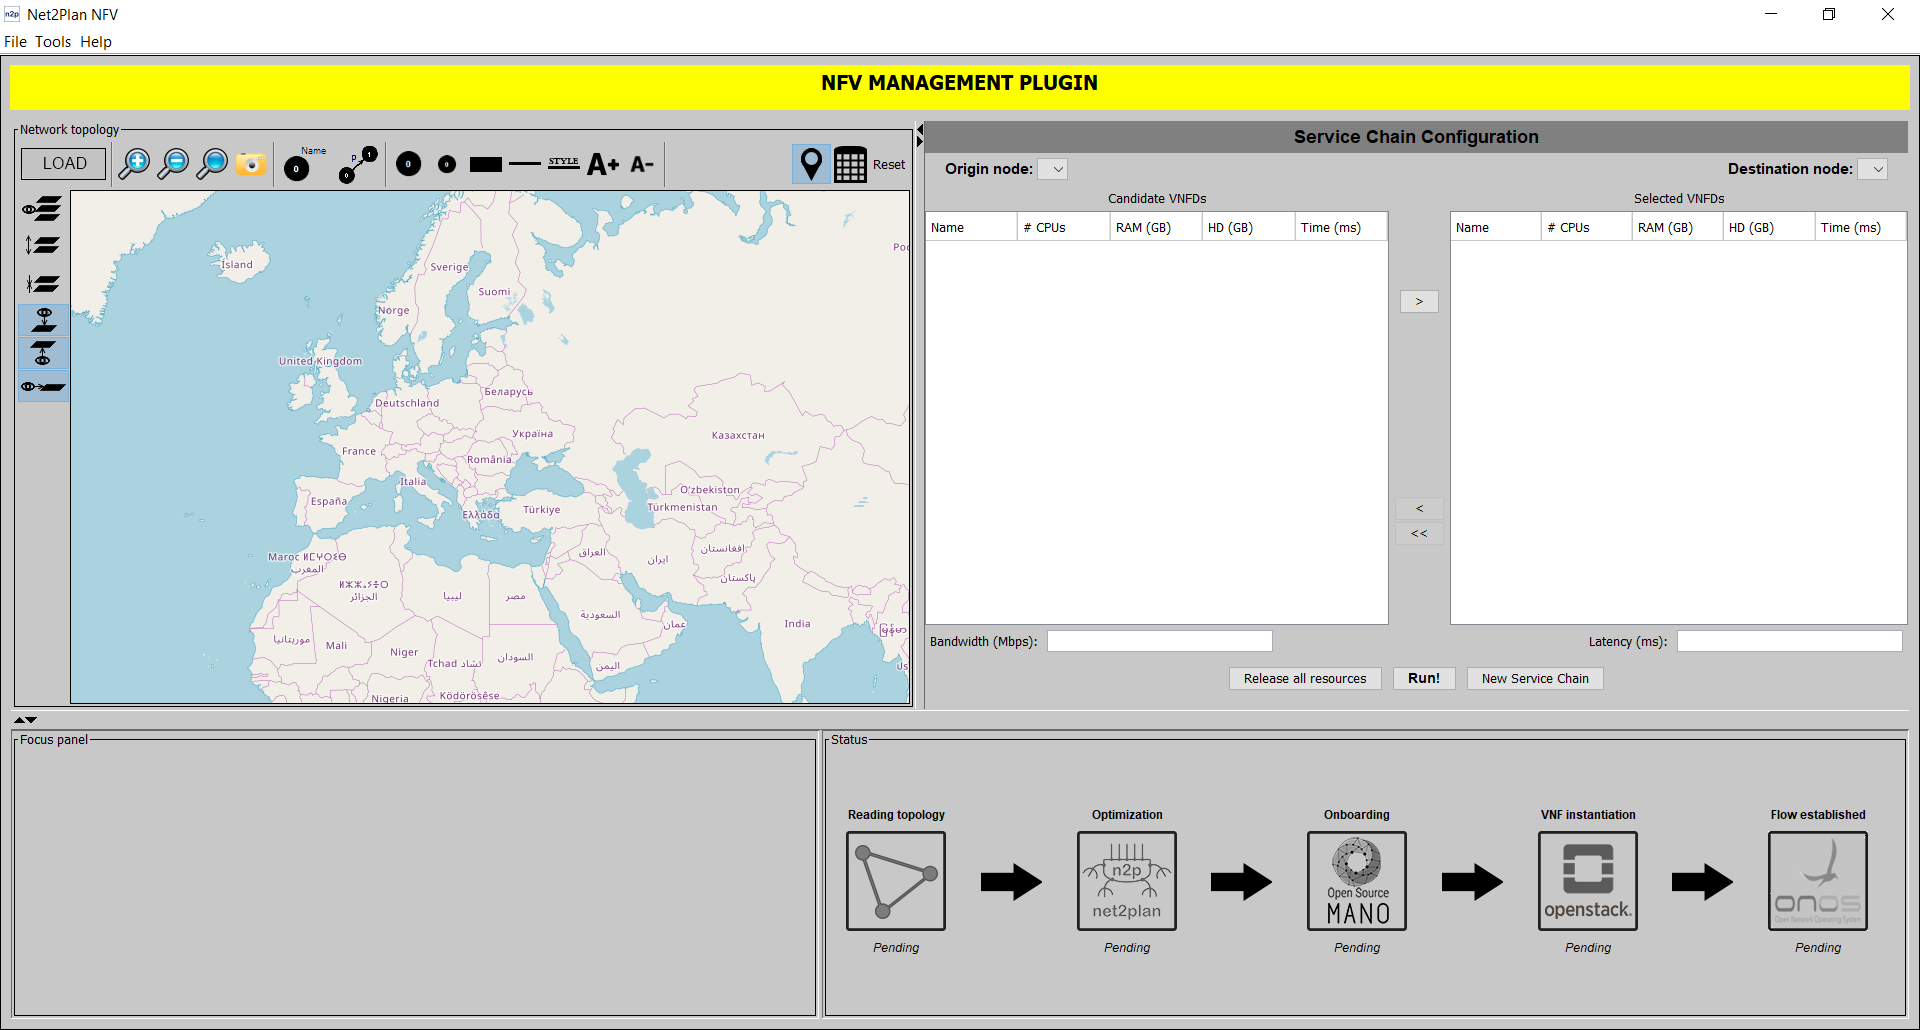
\includegraphics[width=0.7\linewidth]{imagenes/nfvplugin_dashboard}
	\caption{Interfaz gráfica del Plugin al inicio}
	\label{fig:nfvproof_inicio}
\end{figure}

\begin{itemize}
	\item Paso 1. Haciendo click en el botón LOAD, Net2Plan recibe la información referente a la red de transporte de ONOS haciendo uso de ONOSClient, la información sobre los posibles VNFs a instanciar de ETSI-OSM haciendo uso de J-OSMClient y la información sobre cada VIM de OpenStack haciendo uso de OpenStackClient.
	
	\item Paso 2. El usuario define la Service Chain que quiere satisfacer (nodo origen, nodo destino, secuencia ordenada de VNFs a atravesar, latecia máxima y ancho de banda) a través de la interfaz gráfica del Plugin.
	
	\item Paso 3. Net2Plan recibe la información introducida por el usuario y la transfiere al LA-SCCE para que ejecute el algoritmo que devolverá como resultado una ruta de enlaces para la Service Chain y una serie de VNFs instanciadas en diferentes VIMs.
	
		\begin{figure}[!ht]
		\centering
		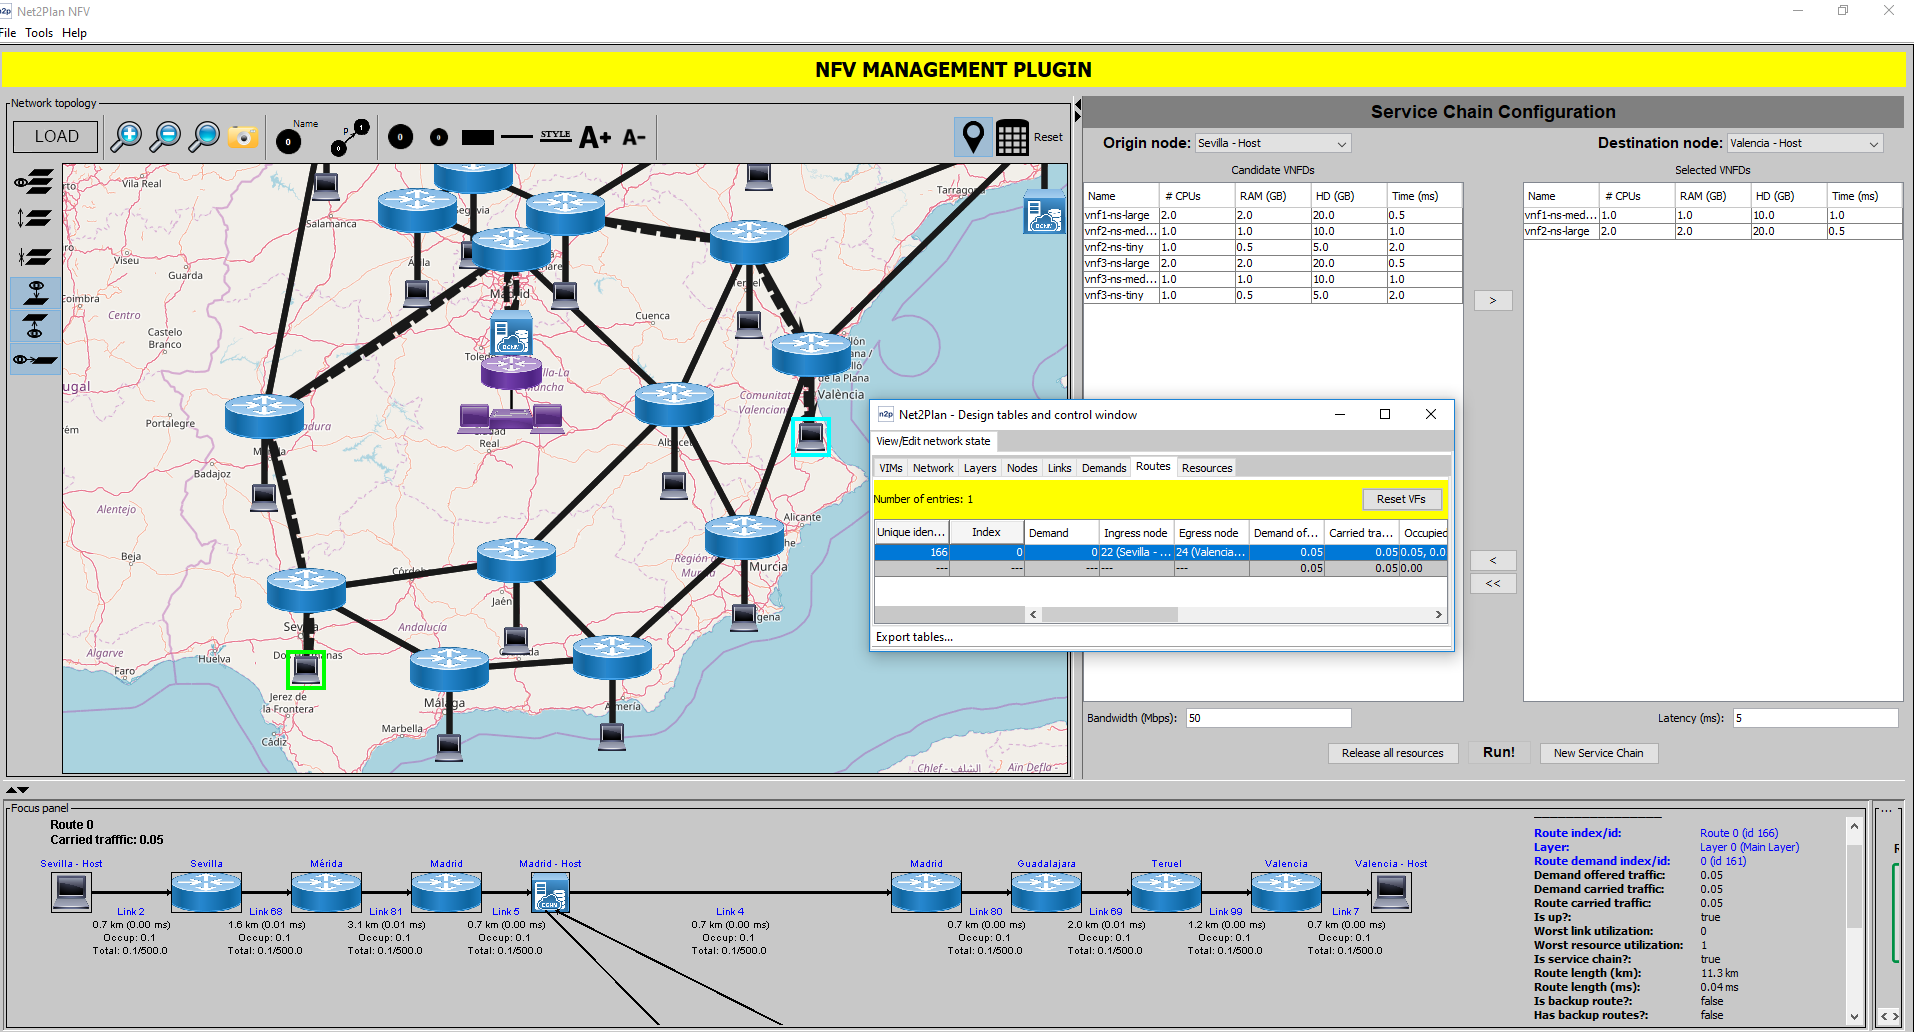
\includegraphics[width=0.7\linewidth]{imagenes/nfv_service_chain}
		\caption{Interfaz gráfica del Plugin con la ruta establecida}
		\label{fig:nfvservicechain}
	\end{figure}
	
	\item Paso 4. Net2Plan envía la orden a ETSI-OSM haciendo uso de J-OSMClient de instanciar las VNFs en los VIMs que el LA-SCCE obtuvo como óptimos.
	
	\begin{figure}[!ht]
		\centering
		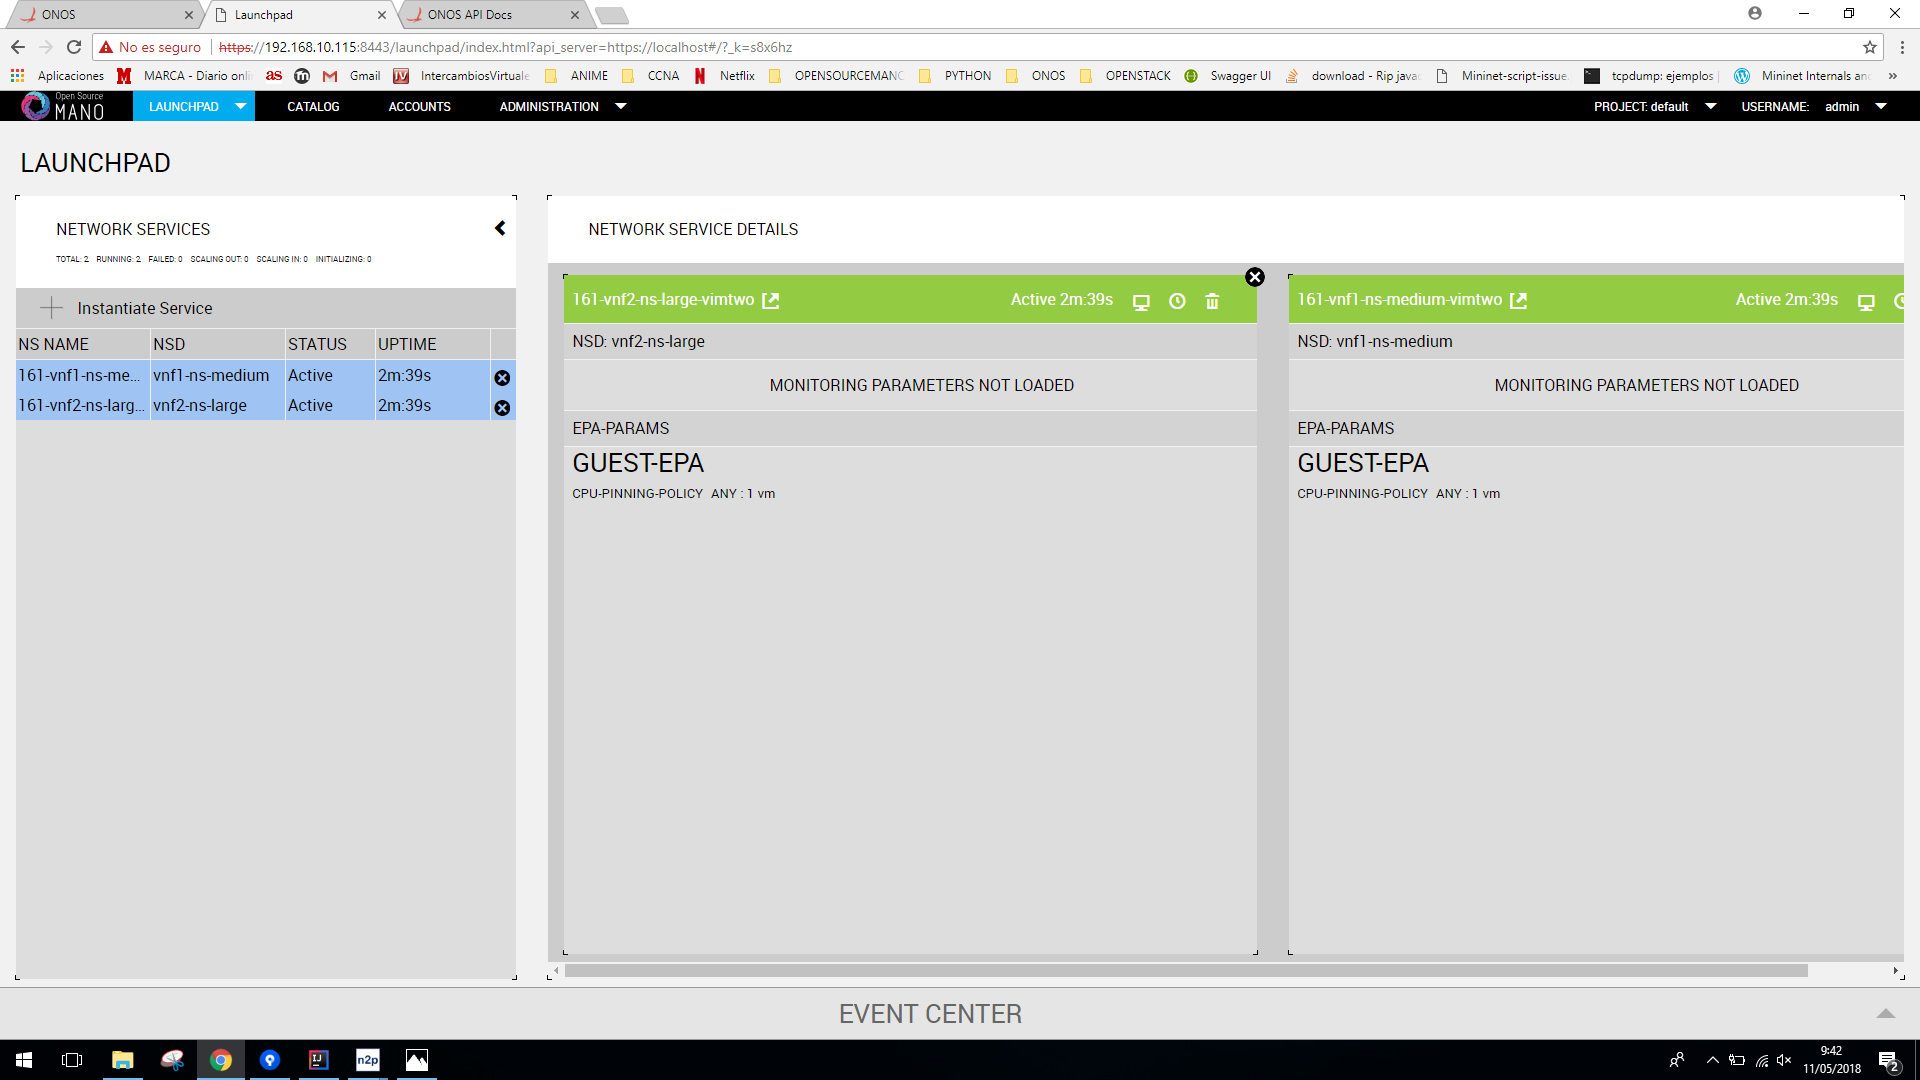
\includegraphics[width=0.7\linewidth]{imagenes/osm_vnfs}
		\caption{Interfaz gráfica de OSM con los VNFs instanciados}
		\label{fig:osmvnfs}
	\end{figure}
	
	
	\item Paso 5. ETSI-OSM envia órdenes a los diferentes VIMs (OpenStack) para que alojen las diferentes máquinas virtuales correspondientes a los VNFs. La comunicacion entre OSM y OpenStack es transparente al usuario.
	
	\item Paso 6. Net2Plan envía la orden a ONOS, haciendo uso de ONOSClient, con diferentes reglas de flujo para establecer en los diferentes switches de la red de transporte, todo según la ruta óptima obtenida por el LA-SCCE.
	
	\begin{figure}[!ht]
		\centering
		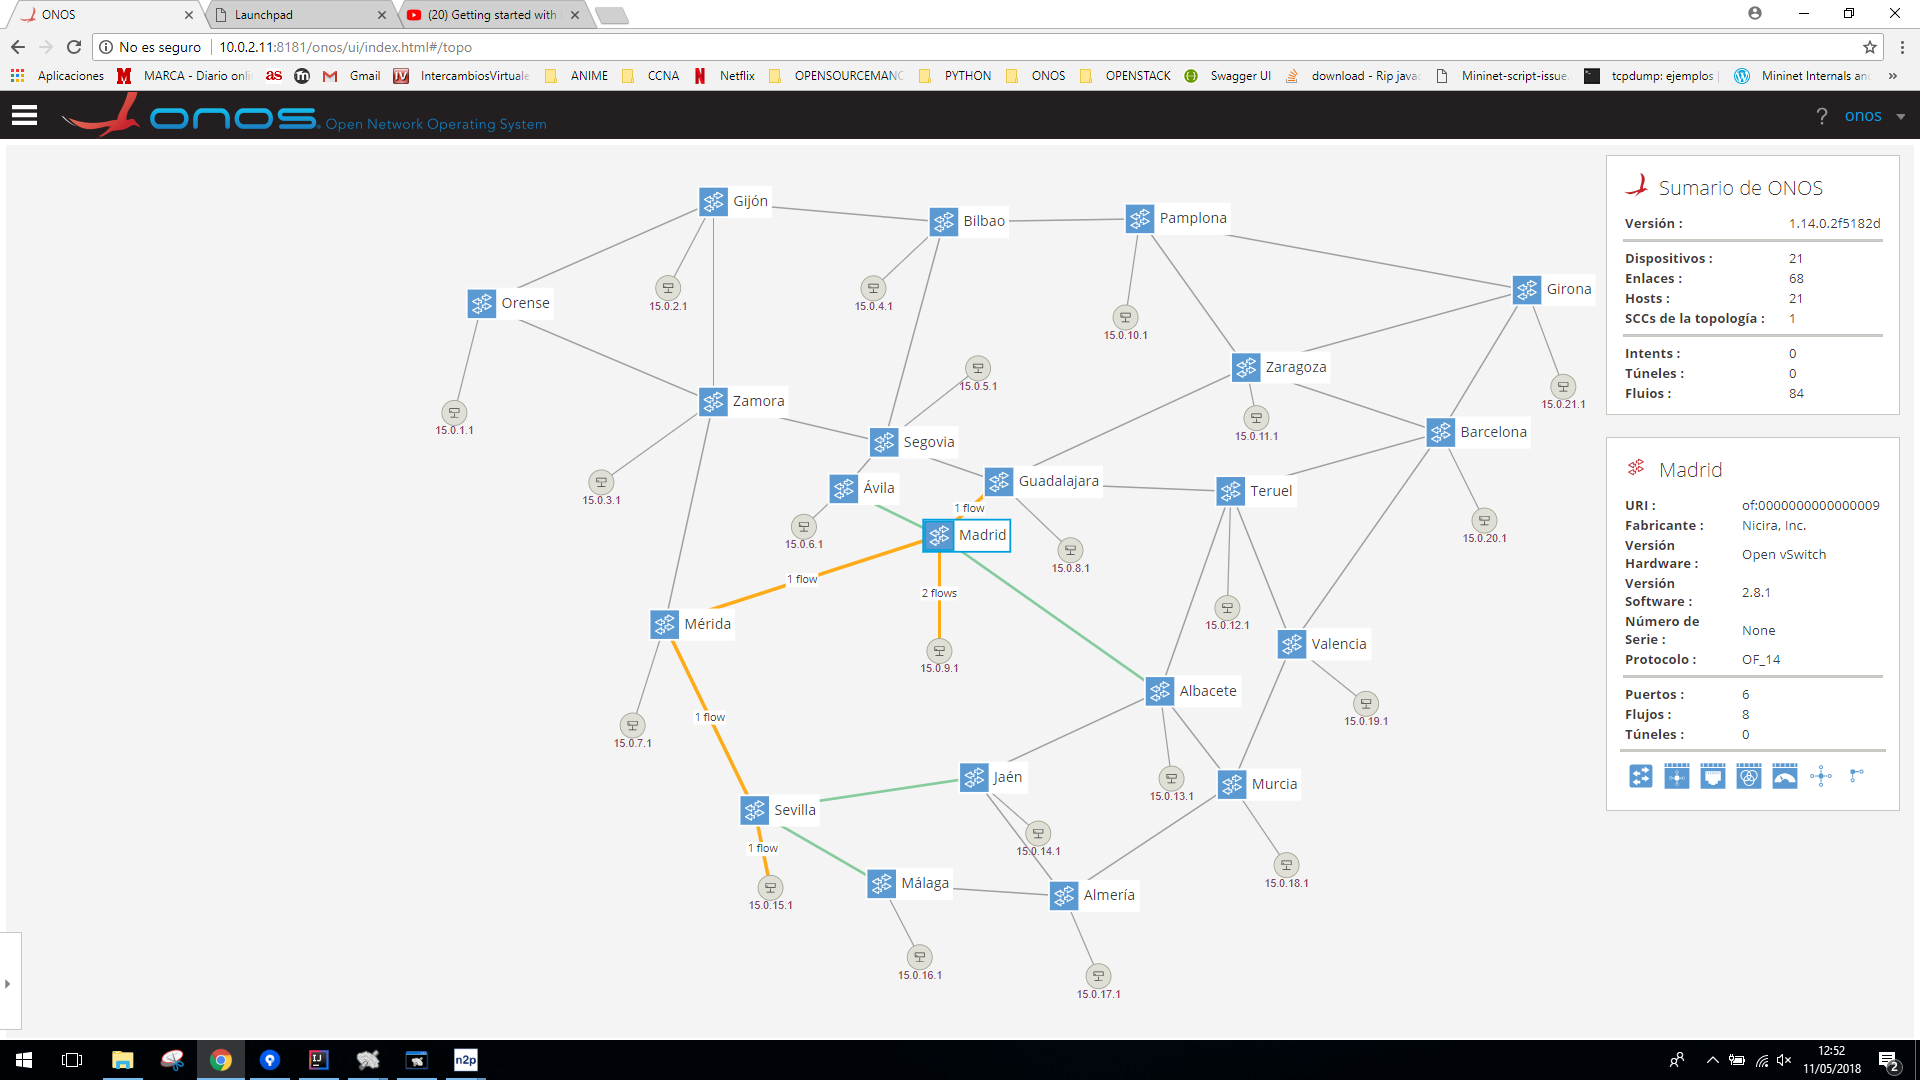
\includegraphics[width=0.7\linewidth]{imagenes/topo_onos}
		\caption{Interfaz gráfica de ONOS con las reglas de flujo establecidas}
		\label{fig:topo_onos}
	\end{figure}

	\clearpage

	\item Paso 7. Una vez establecidos las reglas de flujo mediante OpenFlow, se realiza una prueba de conexión para asegurar que la Service Chain está establecida.
	
	\begin{figure}[!ht]
		\centering
		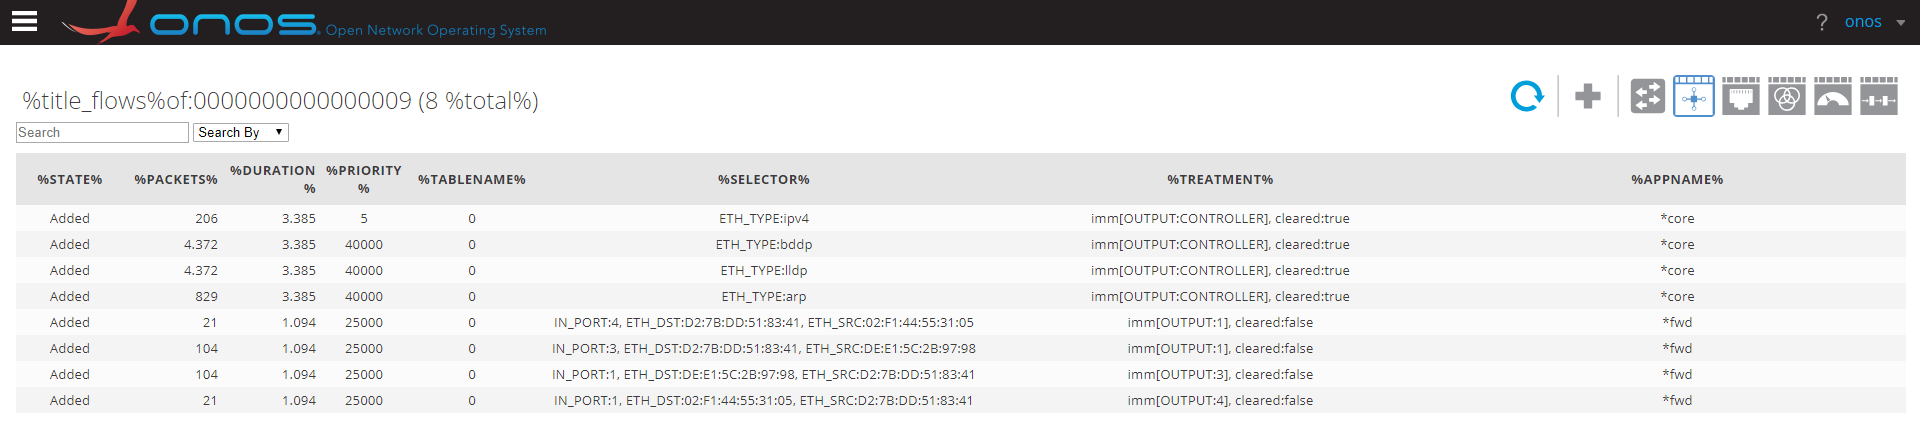
\includegraphics[width=0.7\linewidth]{imagenes/onos_flowrules}
		\caption{Prueba de conectividad en la GUI de ONOS}
		\label{fig:onosflowrules}
	\end{figure}


\end{itemize}

